\documentclass[a4paper,slidestop,xcolor=pst,dvips,blue]{beamer}

\usepackage{beamerthemesplit}
\usepackage[utf8]{inputenc}
\usepackage[spanish]{babel}
\usepackage{graphicx}
\usepackage{pstricks} % PSTricks package
\usepackage{setspace}
\usepackage{multirow}
\usepackage{listings}
\usepackage{pgfpages}
\usepackage{hyperref}
\usepackage{etoolbox}
\usepackage{epstopdf}

\makeatletter
\patchcmd{\beamer@sectionintoc}{\vskip1.5em}{\vskip0.5em}{}{}
\makeatother

\setbeamercovered{dynamic}
\setcounter{tocdepth}{2}
\setbeamercolor{frametitle}{fg=black,bg=white}
\setbeamercolor{section in toc shaded}{fg=black}
\setbeamercolor{section in toc}{fg=red}
\setbeamercolor{subsection in toc shaded}{fg=black}
\setbeamercolor{subsection in toc}{fg=red}
\setbeamerfont{section in toc}{size=\small}
\setbeamerfont{subsection in toc}{size=\small}
\setbeamertemplate{section in toc shaded}[default][99]
\setbeamertemplate{subsection in toc shaded}[default][99]

\AtBeginSection[]
{\begin{frame}[c]
  \frametitle{Índice}
	\tableofcontents[currentsection,
        sectionstyle=show/shaded,
        subsectionstyle=hide]
\end{frame}}

\AtBeginSubsection[]
{\begin{frame}[c]
	\frametitle{Índice}
	\tableofcontents[
  		currentsection,
  		sectionstyle=shaded/shaded,
  		currentsubsection,
  		subsectionstyle=show/shaded/hide
		]
\end{frame}}

\setbeamercolor{frametitle}{fg=black,bg=white}

\setbeamertemplate{frametitle}{
	\begin{centering}
		\insertframetitle
		\par
	\end{centering}
}

\usetheme[secheader]{Boadilla}


\title[Patrones de SIE]{Patrones para el Desarrollo de Arquitecturas Empresariales}

\author[P. Sánchez]{\alert{Pablo Sánchez}}

\institute[IIE]{
		   Dpto. Ingeniería Informática y Electrónica \\
		   Universidad de Cantabria \\
		   Santander (Cantabria, España) \\
		   \texttt{p.sanchez@unican.es}
}

\date{}

\begin{document}

\begin{frame}[c]
	\titlepage
	\begin{columns}
		\column{0.50\linewidth}
			\centering
    		
\includegraphics[width=.28\textwidth,keepaspectratio=true]{images/istr.eps}
		\column{0.50\linewidth}
			\centering
			
\includegraphics[width=.25\textwidth,keepaspectratio=true]{images/uc.eps}
	\end{columns}
\end{frame}

\begin{frame}[c]
    \frametitle{\alert{Advertencia}}
    \begin{center}
        Todo el material contenido en este documento no constituye en modo alguno una obra de referencia o apuntes oficiales mediante el cual se puedan preparar las pruebas evaluables necesarias para superar la asignatura. \ \\
        \ \\
        Este documento contiene exclusivamente una serie de diapositivas cuyo objetivo es servir de complemento visual a las actividades realizadas en el aula para la transmisi{\'o}n del contenido sobre el cual versar{\'a}n las mencionadas pruebas evaluables.  \ \\
        \ \\
        Dicho de forma m{\'a}s clara, \alert{estas transparencias no son apuntes y su objetivo no es servir para que el alumno pueda preparar la asignatura.}
    \end{center}
\end{frame}

\section{Introducción}

\begin{frame}[c]
    \frametitle{Objetivos del Tema}
    \begin{enumerate}[<+->]
         \item Comprender qué es un \emph{Sistema de Información Empresarial (SIE)}.
         \item Comprender y por qué y cómo se divide un sistema empresarial en capas.
         \item Comprender la función de cada capa de un SIE.
         \item Conocer las tecnologías sw que se utilizan para implementar SIE.
         \item Conocer y comprender los patrones existentes para el desarrollo de la \emph{capa de negocio}.
         \item Comprender y saber utilizar la metodología \emph{Domain-Driven Design (DDD)}.
         \item Comprender el problema de la impedancia objeto-relacional.   
         \item Comprender y saber utilizar los patrones para la construcción de un \emph{puente object-relacional}.
         \item Comprender y saber utilizar los patrones existentes para la construcción de la \emph{capa de servicio}.
         \item Conocer los patrones existentes para el desarrollo de la \emph{capa de persistencia}.
    \end{enumerate}
\end{frame}

\begin{frame}[c]
    \frametitle{Bibliografía}
    \begin{thebibliography}{1}

        \bibitem[Fowler, 2002]{Fowler2002x}
        Fowler, M. (2002).
        \newblock {\em {Patterns of Enterprise Application Architecture}}.
        \newblock Addison-Wesley Professional.

        \bibitem[Esposito and Saltarello, 2014]{Esposito2014x}
        Esposito, D. and Saltarello, A. (2014).
        \newblock {\em {Microsoft .NET - Architecting Applications for the
          Enterprise}}.
        \newblock 2 edition.

    \end{thebibliography}
\end{frame}


\begin{frame}[c]
    \frametitle{Bibliografía}
    \begin{thebibliography}{1}

        \bibitem[Schwaber and Sutherland, 2011]{Schwaber2011}
        Schwaber, K. and Sutherland, J. (2011).
        \newblock {The Scrum Guide - The Definitive Guide to Scrum: The Rules of the Game}.

        \bibitem[Cohn, 2004]{Cohn2004}
        Cohn, M. (2004).
        \newblock {\em {User Stories Applied}},
        \newblock Addison-Wesley.

    \end{thebibliography}
\end{frame}

\section{Sistemas y Arquitecturas Empresariales}

\subsection{Sistemas de Información Empresarial}

\begin{frame}
    \frametitle{Sistema de Información Empresarial}
    %% TODO: Buscar una definición mejor o más estandarizada.
    \begin{block}{Sistema de Información  Empresarial (SIE)}
        Un \emph{Sistema de Información Empresarial} es un sistema sw que da soporte a diferentes procesos de negocio de una determinada organización.
    \end{block}
    \uncover<2->{
    \begin{block}{Características de los Sistemas de Información Empresariales}
    \begin{enumerate}
        \item<3-> Necesita almacenar datos, y normalmente, en gran volumen.
        \item<4-> Los datos que almacenan representan un activo importante y duradero en el tiempo.
        \item<5-> Los gestión de los datos debe obedecer a ciertas \emph{reglas de negocio}.
        \item<6-> Las operaciones ejecutadas necesitan ser \emph{transaccionales}.
        \item<7-> Los datos pueden ser accedidos y manipulados de manera concurrente. 
        \item<6-> Utilizan un gran número de interfaces de usuario que pueden requerir de sistemas avanzados de visualización de datos.
        \item<7-> Interoperan con otros Sistemas de Información Empresarial.
    \end{enumerate}
    \end{block}
    }
\end{frame}

\subsection{Sistema de Información Empresarial Web}

%% TODO : Añadir definición de Sistema Web 

\begin{frame}[c]
	\frametitle{¿Por qué se utilizan tecnologías Web?}
    \centering \textbf{Ventajas} \\
    \begin{enumerate}
        \item<2-> Multiplataforma.
        \item<3-> Onmipresencia de la web.
        \item<4-> No precisan permisos especiales a nivel de red.
        \item<5-> Facilidad de mantenimiento.
        \item<6-> Fuerte estandarización.
        %% Balanceadores de carga
        \item<7-> Favorecen la \emph{recognizability}, reduciendo su curva de aprendizaje.
        \item<8-> Madurez de las herramientas.
    \end{enumerate}
    \uncover<9->{
        \centering \textbf{Inconvenientes} \\
        \begin{enumerate}
            \item<10-> Seguridad.
            %% https://goo.gl/ypz4VD
            \item<11-> Tecnologías originalmente desarrolladas para \emph{hipertexto}.
            \item<12-> Tecnologías lentas.
            \item<13-> Tecnologías dependientes de terceros.
        \end{enumerate}
    }
}

\subsection{Arquitecturas Empresariales en Capas}

\begin{frame}[c]
	\frametitle{Arquitectura en Capas de un Sistema de Información Empresarial}
    %% TODO: Revisar arquitectura para eliminar referencias a patrones específicos.
	\begin{center}
        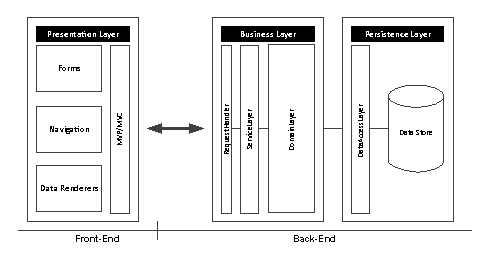
\includegraphics[width=\linewidth,keepaspectratio=true]{images/enterpriseLayers/enterpriseLayers.eps}
	\end{center}
\end{frame}

%% TODO: Añadir ejemplo de sistema monolítico.

\begin{frame}[c]
	\frametitle{Responsabilidades de la Capa de Presentación}
	\begin{enumerate}[<+->]
        \item Permitir a los usuarios interactuar con el sistema.
        \item Introducir datos en el sistema (validándolos previamente).
        \item Visualizar los datos de salida de manera amigable al usuario.
        \item Facilitar operaciones simples (filtros, ordenaciones y cambios de formato) sobre los datos.
        \item Facilitar la navegación por el sistema.
        \item Mejorar la experiencia de usuario (UX). %% Hellmans
        \item Gestionar la comunicación con el servidor.
        \item Gestionar situaciones excepcionales.
	\end{enumerate}
\end{frame}

\begin{frame}[c]
	\frametitle{Responsabilidades de la Capa de Negocio}
	\begin{enumerate}[<+->]
        \item Atender las peticiones de los clientes.
        \item Asegurar el cumplimiento de \alert{reglas de negocio} existentes.
        \item Asegurar la \alert{transaccionalidad} de las operaciones de negocio.
        \item Validar las peticiones de los clientes.
        \item Recuperar y almacenar datos del almacén o almacenes persistentes.
        \item Facilitar la eficiencia del sistema.
        \item Ayudar a mejorar la experiencia de usuario.
        \item Controlar el acceso a los datos.
        \item Gestionar la comunicación con los servicios externos.
        \item Ejecutar operaciones del sistema.
        \item Gestionar de manera adecuada casos excepcionales.
	\end{enumerate}
\end{frame}

\begin{frame}[c]
	\frametitle{Responsabilidades de la Capa de Persistencia}
	\begin{enumerate}[<+->]
        \item Almacenar los datos de manera no volátil.
        \item Recuperar datos del almacén persistente,
        \item Asegurar la disponibilidad de los datos.
        \item Controlar la integridad de los datos.
        \item Asegurar un acceso eficiente a los datos.
	\end{enumerate}
\end{frame}

\subsection{Tecnologías de Implementación para Arquitecturas Empresariales}

\begin{frame}[c]
	\frametitle{Tecnologías de Implementación ES}
    %%  Dividir en tres imágenes
	\begin{center}
        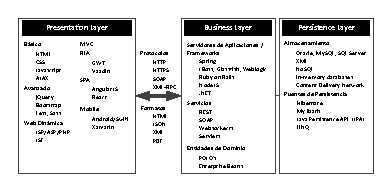
\includegraphics[width=\linewidth,keepaspectratio=true]{images/enterpriseLayers/technologies.eps}
	\end{center}
\end{frame}

%\subsection{Distribución de Capas en Arquitecturas Empresariales}
%
%\begin{frame}[c]
%	\frametitle{Despliegue de Aplicaciones Empresariales}
%	\begin{enumerate}[<+->]
%        \item Front-end en el cliente y back-end en uno o más servidores.
%        \item Dominio y persistencia pueden ir en el mismo servidor (\emph{two tier}) o en servidores separados (three tiers).
%        \item Trabajo con conexión puede requerir parte de la capa de dominio (y persistencia) en el cliente.
%        \item Los clientes pueden ser pesados (PCs) o ligeros (Smartphones, tablets).
%        \item La capa de presentación puede ser de código fijo (app, desktop) o móvil (HTML + Javascript).
%        %% Añadir que parte de la capa de presentación puede ir en el servidor.
%	\end{enumerate}
%\end{frame}

\section{Capa de Negocio}

\subsection{Table Module}

\subsection{Transaction Script}

\subsection{Domain Model}

\section{Domain-Driven Design}

\begin{frame}[c]
	\frametitle{Domain-Driven Design}
	\begin{block}{Principio Básico Domain-Driven Design}
        Las tecnologías van y vienen, los negocios (dominios) permanecen.
	\end{block}
\end{frame}

\begin{frame}[c]
	\frametitle{Domain-Driven Design}
    \begin{block}{Elementos de Domain-Driven Design}
        \begin{enumerate}[<+->]
              \item Ubiquitous language.
            \item Bounded Context.
            \item Context or Strategic Map.
            \item Value Objects.
            \item Entities.
            \item Modules.
            \item Aggregate and Aggregate Roots.
            \item Repositories.
            \item Services.
            \item Factorías.
        \end{enumerate}
    \end{block}
\end{frame}


\section{Sumario y Referencias}

\begin{frame}[c]
    \frametitle{¿Qué Tengo que Saber de Todo Esto?}
    \begin{enumerate}[<+->]
        \item
    \end{enumerate}
\end{frame}

%\subsection{Referencias}
%
%\begin{frame}
%	\frametitle{Referencias}
%    \nocite{}
%	\bibliographystyle{apalike}
%    \bibliography{arqEmp}
%\end{frame}

\end{document}
